\chapter{アクセラレータの評価}
\section{評価環境}
今回実装するアクセラレータは表\ref{evalu}に示す環境で設計を行い、評価を行った。
Vivado HLSはXilinx社の提供する高位合成ツールで、畳み込みアクセラレータのシミュレーションは
このツール上で行った。評価ボードとFPGAにはFiC-SW1ボードのものと同様にKintex UltraScale XCKU095を用いた。

また、比較のためにCPUで畳み込み演算のソフトウェア実行を行った。そのときのソフトウェア実行環境を表\ref{evacpu}に
示す。

\begin{table}[ht]
 \begin{center}
  \caption{CNNアクセラレータの評価環境}
   \begin{tabular}{|c|c|} \hline
     ツール & Vivado HLS Version 2016.1 (Xilinx) \\ \hline
     評価ボード & Kintex UltraScale XCKU095 (Xilinx) \\ \hline
     FPGA & XCKU095-FFVB2104 (Xilinx) \\ \hline
  \end{tabular}
  \label{evalu}  
 \end{center}
\end{table}

\begin{table}[ht]
 \begin{center}
  \caption{ソフトウェア実行環境}
   \begin{tabular}{|c|c|} \hline
     CPU & Intel Core i5-4250U \\ \hline
     動作周波数 & 1.30GHz \\ \hline
     コンパイラ & GCC 4.4.7 20120313 \\ \hline
  \end{tabular}
  \label{evacpu}  
 \end{center}
\end{table}

\section{アクセラレータのクロックサイクル数とリソース消費量}
演算モジュールの演算器サイズを(Tm, Tn)= (24, 8)としたときの各畳み込み層の計算時間を測定した。
Tmは畳み込み層5層のなかでのMの最大値である24を、Tnは予想されるリソース消費量が上限以下になるように暫定的に決定した。
表\ref{tdmtime}からノード数を16より大きくすると通信時間が増えることがわかるため、今回の実装では通信時間が最小の条件下でノード数が最も高い16並列時を取り扱う。

表\ref{cnnexe}は、CONV1からCONV5を16並列で計算した際のサイクル数の結果となる。
特に、入出力特徴マップのサイズが大きく、次元数が低いCONV1が508118サイクルと最もクロックサイクル数が大きい。
今回のアクセラレータは入出力の特徴マップの次元数以上に処理を並列化していない設計のため、このような結果となったと考えられる。

また、このときのリソース消費量を図\ref{gra_resource}に示す。表\ref{resource}は図\ref{gra_resource}の詳細な結果である。
それぞれの畳み込み層のアクセラレータのリソース消費量は上限に収まっているため、(Tm, Tn)=(24, 8)の演算モジュールのサイズは(最適とはいかないまでも)妥当な値であったと言える。
ただし、単純にアクセラレータを5層分実装するにはリソースが足りないため、各アクセラレータの(Tm, Tn)を調節して規模を縮小させるか、リソース共有を行うクロスレイヤーな設計を考える必要がある。

\begin{table}[ht]
 \begin{center}
  \caption{16並列時の畳み込みアクセラレータの演算サイクル数}
   \begin{tabular}{|c|c|} \hline
     & サイクル数 \\ \hline
     CONV1 & 508118 \\
     CONV2 & 409746 \\
     CONV3 & 166554 \\
     CONV4 & 245434 \\
     CONV5 & 242506 \\ \hline
  \end{tabular}
  \label{cnnexe}  
 \end{center}
\end{table}

\begin{table}[ht]
 \begin{center}
  \caption{16並列時の畳み込みアクセラレータのリソース消費量}
   \begin{tabular}{|c|c|c|c|c|} \hline
     & BRAM 18K & DSP48E & FF & LUT \\ \hline
     CONV1 & 903 & 32 & 11388 & 181047 \\
     CONV2 & 496 & 66 & 80886 & 249112 \\
     CONV3 & 664 & 98 & 135466 & 290533 \\
     CONV4 & 736 & 98 & 152868 & 321012 \\
     CONV5 & 504 & 66 & 119670 & 244851 \\ \hline
     Avaiable & 3360 & 768 & 1075200 & 537600 \\ \hline
  \end{tabular}
  \label{resource}  
 \end{center}
\end{table}

\begin{figure}[ht]  
 \begin{center}   
	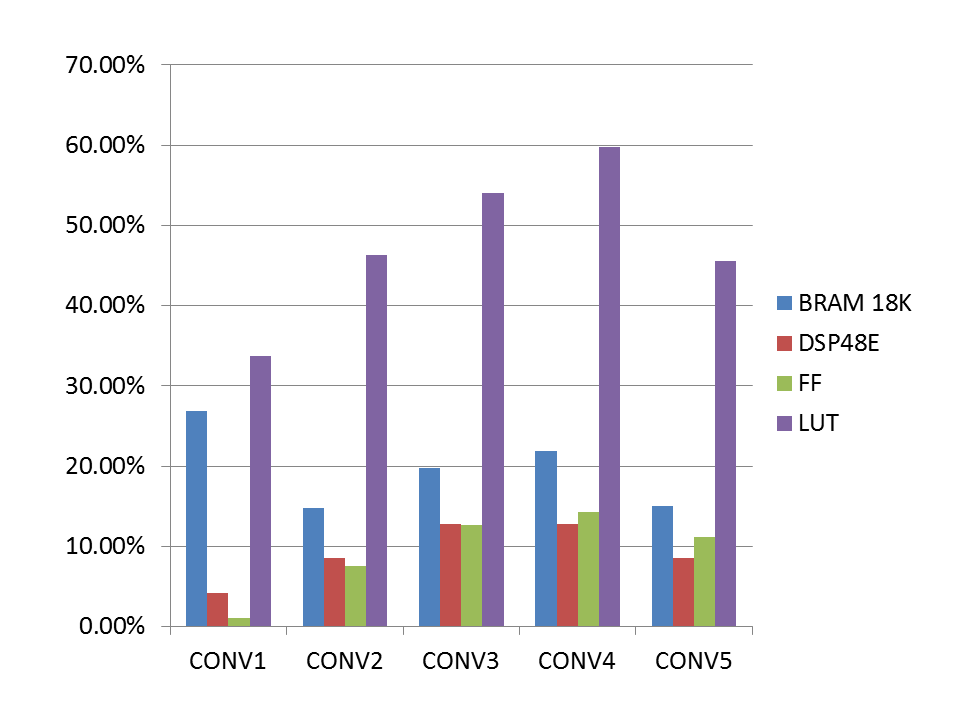
\includegraphics[width=1.0\columnwidth,bb=0 0 720 540]{img/resource.png}
  \caption{16並列時の畳み込みアクセラレータのリソース割合}
%  \ecaption{Static analysis result of an example pattern}
  \label{gra_resource}  
 \end{center}  
\end{figure}


\section{FiC-SW1での畳み込み層の計算時間と通信時間}
FiC-SW1上のKintex UltraScale KU095は100MHzで動作するため、クロックサイクル数から計算時間を計算できる。表\ref{cnnexe}と表\ref{tdmtime}から、16並列時の畳み込み層の計算時間と通信時間の比較を、図\ref{gra_time}に算出した。
表\ref{timecomp}は図\ref{gra_time}の詳細な結果である。
通信時間に対する計算時間の比率は、約2倍から約10倍、CONV5から識別層FC6の間では約26倍になるという結果になった。CONV5の比率が高くなっているのは、CONV5からFC6の間でプーリング層POOL5によって
特徴マップのデータが大幅に削減され、特徴アップ共有の通信にかかる時間が短縮されたことが原因である。

通信時間の計算には、ネットワークのトポロジ、スイッチの遅延、ヘッダ付与による帯域減少は考慮していないため、実際の通信時間は今回の試算より大きくなると予測される。
また、今回のアクセラレータは単純な設計なため、より複雑で高性能な設計(ストリーム機構の見直し、ダブルバッファの導入など)を施すことで実行サイクル数も小さくできる可能性が残っている。
それに伴って通信時間に対する計算時間の比率も小さくなると推測される。

計算時間と通信時間の合計が畳み込み演算の実行時間である。図\ref{gra_cputime}では、今回のFiC-SW1の畳み込みアクセラーレータでの実行時間と、一般的なCPUやUCLAのマルチレイヤー
CNNアクセラレータでの実行時間と比較した。表\ref{cputime}は図\ref{gra_cputime}の詳細な結果である。CPUでのソフトウェア実行は表\ref{evacpu}に従い、Intel Core i5-4250U(1.60GHz)を使用した。FiC-SW1の畳み込みアクセラレータは、CPUに比べて658倍高速であることがわかる。
これはUCLAの設計\cite{fpgaopt}と比べて半分程度の性能に留まる。しかし、今回の設計ではUCLAが行っているような演算器サイズやバッファリングの最適化は一切行っておらず、
これを行うことで性能が大きく向上する可能性が残っている。アクセラレータの最適化は今後の重要な課題とする。

\begin{table}[ht]
 \begin{center}
  \caption{16並列時の通信時間に対する計算時間の比率}
   \begin{tabular}{|c|c|c|c|} \hline
     &  計算時間($\mu$sec) & 通信時間($\mu$sec) & 比率 \\ \hline
     CONV1 &  5081.18 & 699.84 & 7.26 \\
     CONV2 &  4097.46 & 432.64 &  9.47 \\
     CONV3 &  1665.54 & 648.96 &  2.57 \\
     CONV4 &  2454.34 & 648.96 &  3.78 \\
     CONV5 &  2425.06 & 92.16 &  26.31 \\ \hline
  \end{tabular}
  \label{timecomp}  
 \end{center}
\end{table}

\begin{table}[ht]
 \begin{center}
  \caption{畳み込み演算の実行時間}
   \begin{tabular}{|c|c|c|c|} \hline
     &  CPU(msec) & UCLA\cite{fpgaopt}(msec) & FiC-SW1(msec) \\ \hline
     CONV1 & 1110 (192.01x) & 3.66 (0.63x) & 5.78 \\
     CONV2 & 5170 (1141.26x) & 2.37 (0.52x) & 4.53 \\
     CONV3 & 1520 (656.73x) & 1.60 (0.69x) & 2.31 \\
     CONV4 & 2530 (815.26x) & 1.20 (0.39x) & 3.10 \\
     CONV5 & 1670 (663.43x) & 0.80 (0.32x) & 2.52 \\ \hline
     Sum & 12000 (657.67x) & 9.64 (0.53x) & 18.25 \\ \hline
  \end{tabular}
  \label{cputime}  
 \end{center}
\end{table}

\begin{figure}[ht]  
 \begin{center}   
	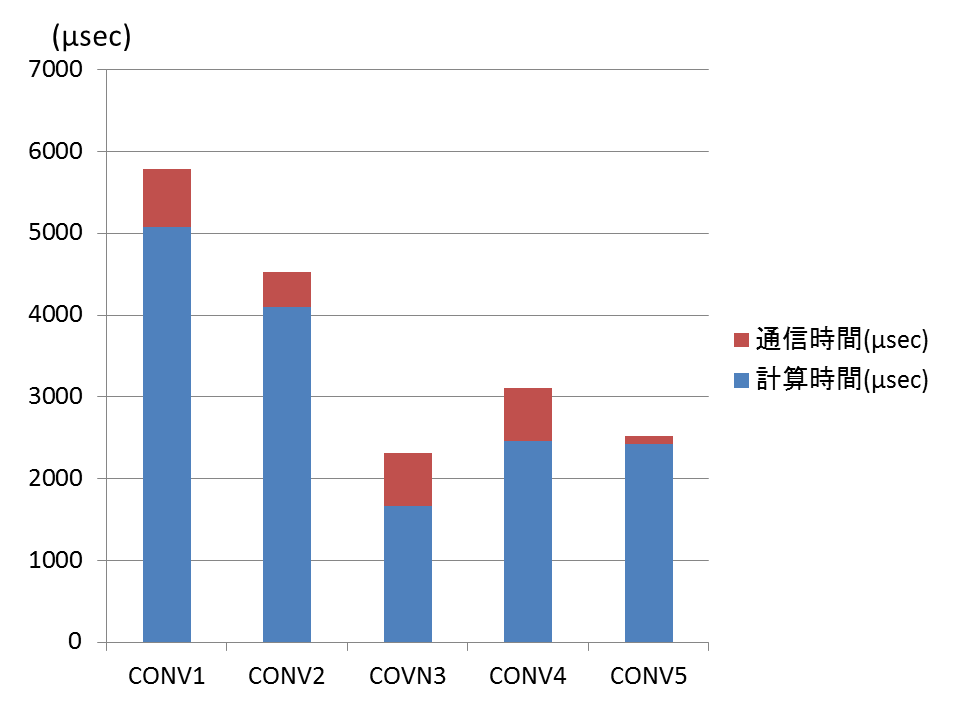
\includegraphics[width=1.0\columnwidth,bb=0 0 720 540]{img/time.png}
  \caption{16並列時の畳み込み層の計算時間と通信時間の比較}
%  \ecaption{Static analysis result of an example pattern}
  \label{gra_time}  
 \end{center}  
\end{figure}

\begin{figure}[ht]  
 \begin{center}   
	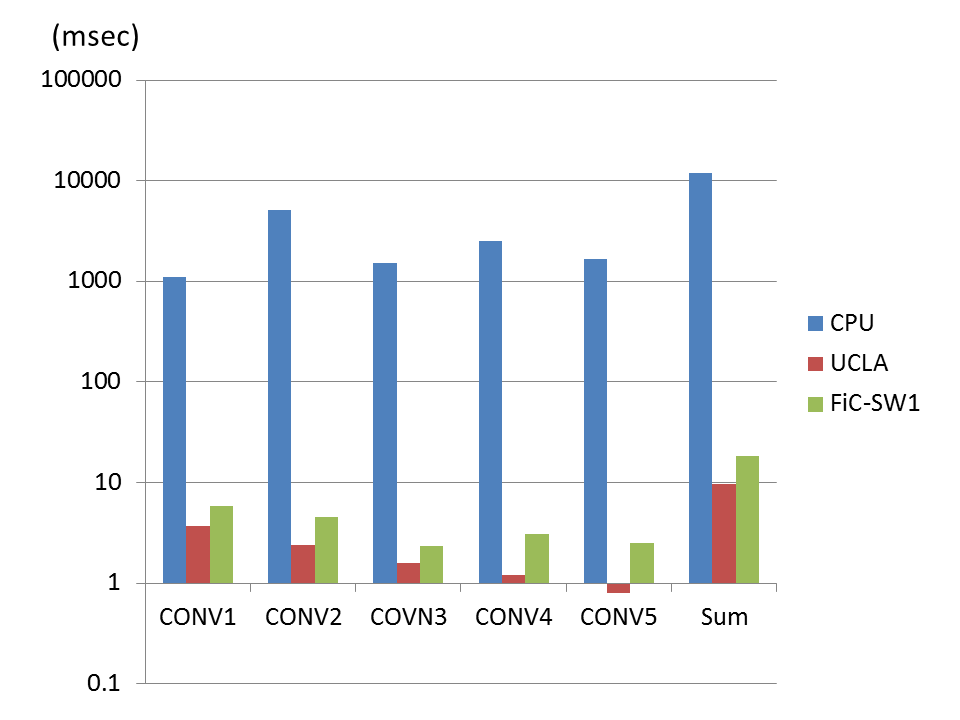
\includegraphics[width=1.0\columnwidth,bb=0 0 720 540]{img/cputime.png}
  \caption{畳み込み演算の実行時間の比較}
%  \ecaption{Static analysis result of an example pattern}
  \label{gra_cputime}  
 \end{center}  
\end{figure}


